\section{Appendices}\label{sec:app:app}

\subsection{Description of simulation, synthesis and hardware tests}\label{sec:app:app_e}

Workflow for simulation and synthesis of firmware is described in \href{\gitbranch/README.md}{\texttt{README}} file.\\\\
List of useful TDF routines and commands for hardware tests:
\begin{itemize}
\item Check crate status\\
\greybox{\$ tdf run crate\_status}
\item Enable TTC signals on AMC13 for all MP7 modules\\
\greybox{\$ tdf run ttc\_enable}
\item Check lock of BC0 and LHC clock\\
\greybox{\$ tdf unittest <module> default}
\item Reset module\\
\greybox{\$ tdf mp7butler reset <module> --clksrc external --clkcfg default-ext}
\item Load firmware to scansd card on all MP7 modules [and load it into FPGAs]\\
\greybox{\$ tdf run uploadfw\_gt <tar file path> [--rebootfpga]}
\item Load firmware from scansd card into FPGAs\\
\greybox{\$ tdf run loadfw\_gt <fw build nr> <nr modules>}
\item Compare hardware results with test vector pattern (for a certain firmware build)\\
\greybox{\$ tdf run multiboard\_function\_test -h}
\item Setup links (GTHs)\\
\greybox{\$ tdf mp7butler rxmgts <module> -e <links>}
\item Align links (GTHs)\\
\greybox{\$ tdf mp7butler rxalign <module> -e <links> [--to-bx <alignment point>]}
\item Check minipods\\
\greybox{\$ tdf mp7butler minipods <module>}
\item ... (other routines are available in /nfshome0/ugtdev/software/tdf/etc/routines)
\end{itemize}

\clearpage
\subsection{Configuration of GTHs}\label{sec:app:app_a}

The FPGA on MP7 board receives and transmits data via GTH transceivers.\\
In Figure~\ref{fig:app:gth_conf} configuration of GTHs~\cite{GTHs} for Global Trigger is shown.

\begin{figure}[htb]
\centering
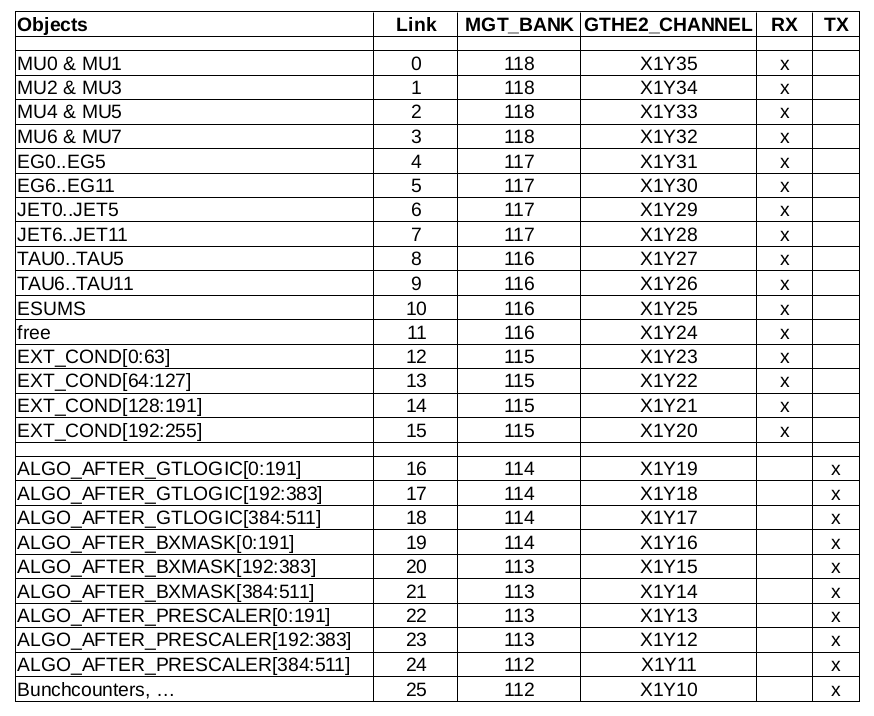
\includegraphics[width=15cm]{figures/gth_xc7v690t_ffg1927}
\caption{Configuration of GTHs}
\label{fig:app:gth_conf}
\end{figure}

\clearpage

\subsection{Configuration of optical input links}\label{sec:app:app_b}

Figure~\ref{fig:app:ugt_inputs} shows the configuration of optical links to Global Trigger.\\
Links 0..3 contains muon data from GMT, links 4..11 data from GCT and links 12..15 external conditions
from AMC502 boards.

\begin{figure}[htb]
\centering
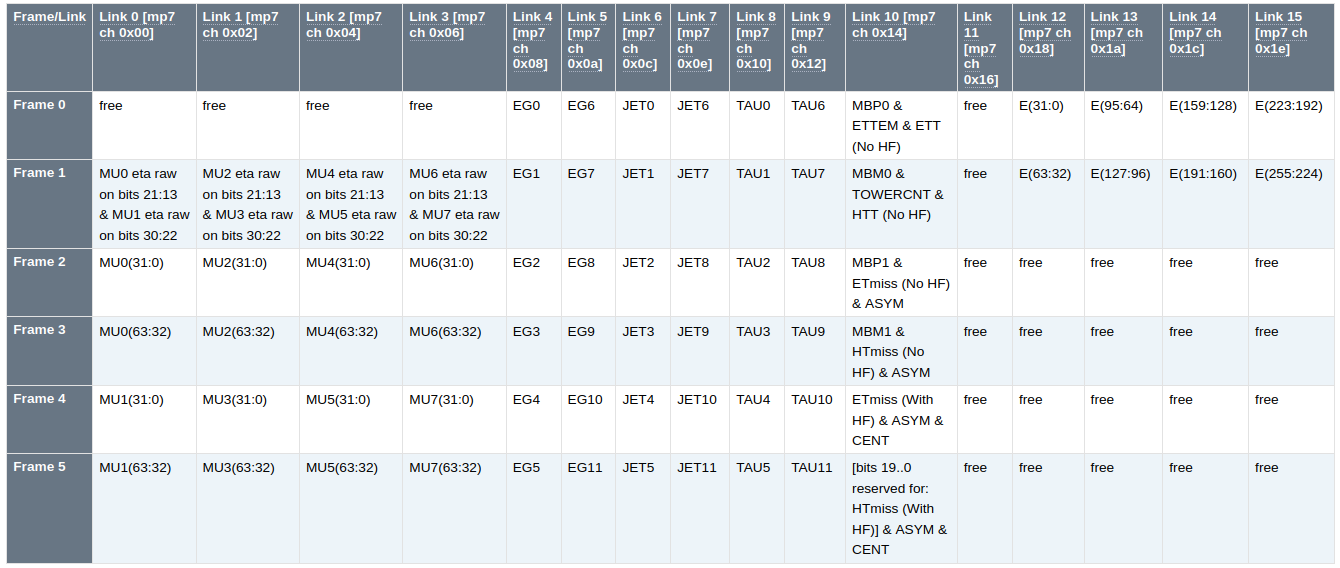
\includegraphics[width=15cm]{figures/ugt_inputs}
\caption{Optical link inputs to Global Trigger}
\label{fig:app:ugt_inputs}
\end{figure}

\subsection{Configuration of links to AMC13 (readout)}\label{sec:app:app_c}

Figure~\ref{fig:app:ugt_outputs} shows the configuration of links from Global Trigger to AMC13 (readout).\\
Links 16..24 contains algo data (after GTL, after BX mask and after prescalers), link 25 contains several counter values.

\begin{figure}[htb]
\centering
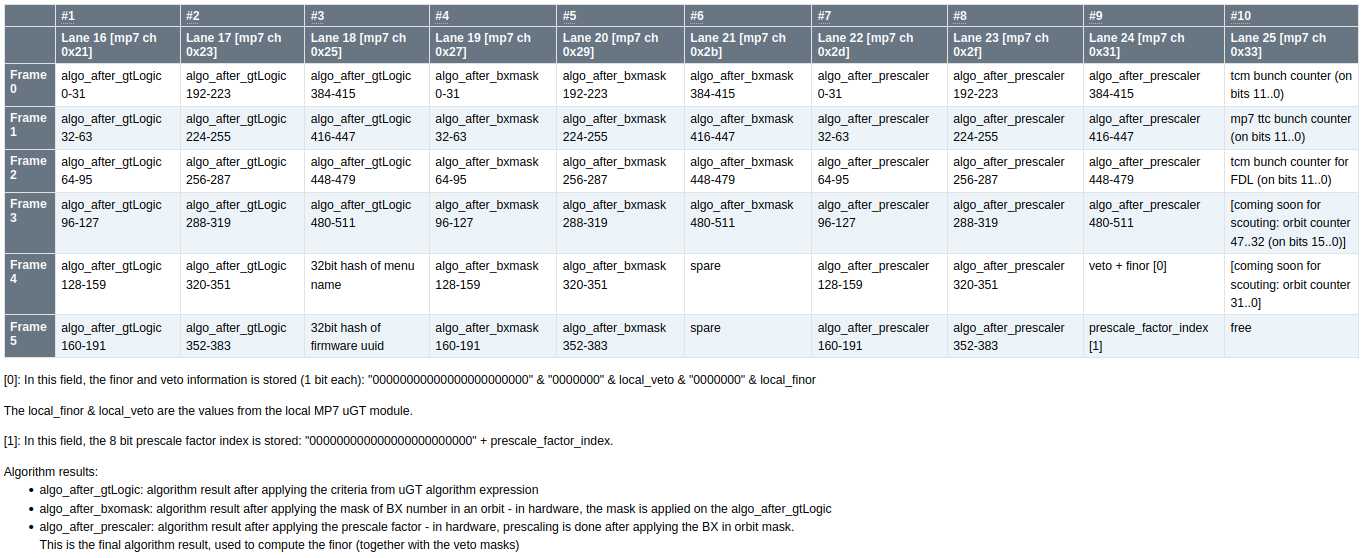
\includegraphics[width=15cm]{figures/ugt_outputs}
\caption{Outputs from Global Trigger to AMC13}
\label{fig:app:ugt_outputs}
\end{figure}

\clearpage

\subsection{Optical patch panel}\label{sec:app:app_d}

Figure~\ref{fig:app:ugt_pp} shows the connections on Global Trigger patch panel for optical links.

\begin{figure}[htb]
\centering
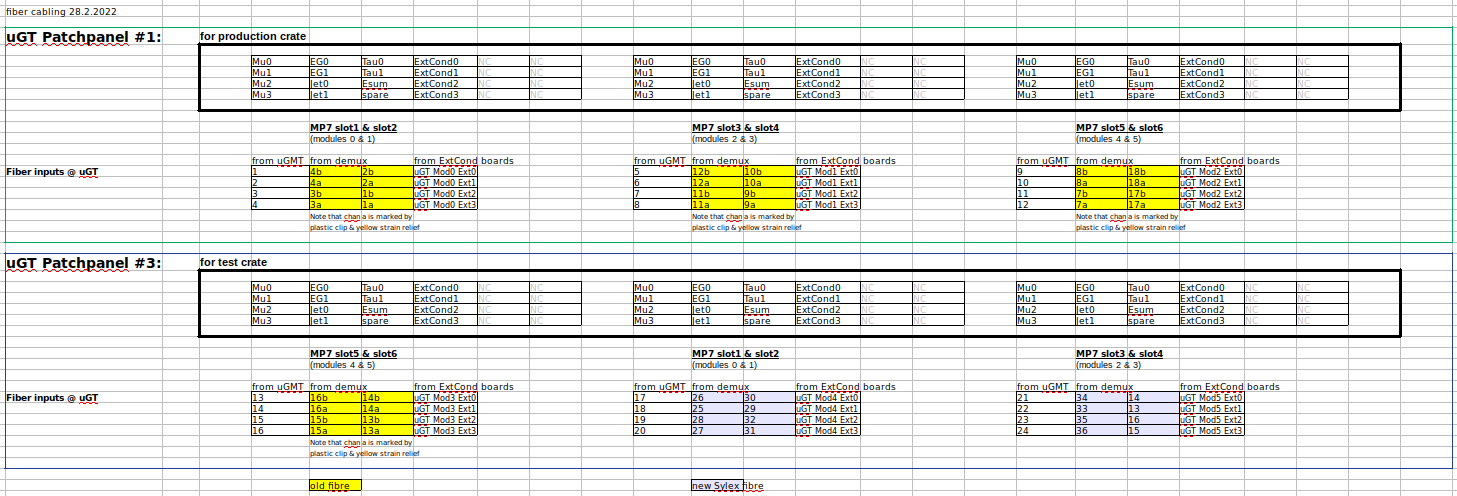
\includegraphics[width=15cm]{figures/ugt_patchpanel}
\caption{Global Trigger patch panel for optical link}
\label{fig:app:ugt_pp}
\end{figure}

\subsection{Description of simulation, synthesis and hardware tests}\label{sec:app:app_e}

Workflow for simulation and synthesis of firmware is described in \href{\gitbranch/README.md}{\texttt{README}} file.\\\\
List of useful TDF routines and commands for hardware tests:
\begin{itemize}
\item Check crate status\\
\greybox{\$ tdf run crate\_status}
\item Enable TTC signals on AMC13 for all MP7 modules\\
\greybox{\$ tdf run ttc\_enable}
\item Check lock of BC0 and LHC clock\\
\greybox{\$ tdf unittest <module> default}
\item Reset module\\
\greybox{\$ tdf mp7butler reset <module> --clksrc external --clkcfg default-ext}
\item Load firmware to scansd card on all MP7 modules [and load it into FPGAs]\\
\greybox{\$ tdf run uploadfw\_gt <tar file path> [--rebootfpga]}
\item Load firmware from scansd card into FPGAs\\
\greybox{\$ tdf run loadfw\_gt <fw build nr> <nr modules>}
\item Compare hardware results with test vector pattern (for a certain firmware build)\\
\greybox{\$ tdf run multiboard\_function\_test -h}
\item Setup links (GTHs)\\
\greybox{\$ tdf mp7butler rxmgts <module> -e <links>}
\item Align links (GTHs)\\
\greybox{\$ tdf mp7butler rxalign <module> -e <links> [--to-bx <alignment point>]}
\item Check minipods\\
\greybox{\$ tdf mp7butler minipods <module>}
\item ... (other routines are available in /nfshome0/ugtdev/software/tdf/etc/routines)
\end{itemize}

\clearpage
